%%%%%%%%%%%%%%%%%%%%%%%%%%%%%%%%%%%%%%%%%%%%%%%%%%%%%%%%%%%%%%%%%%%%%%%%%%%%%%%%
%2345678901234567890123456789012345678901234567890123456789012345678901234567890
%        1         2         3         4         5         6         7         8

\documentclass[letterpaper, 10 pt, conference]{ieeeconf}  % Comment this line out if you need a4paper

%\documentclass[a4paper, 10pt, conference]{ieeeconf}      % Use this line for a4 paper

%\IEEEoverridecommandlockouts                              % This command is only needed if 
                                                          % you want to use the \thanks command

\overrideIEEEmargins                                      % Needed to meet printer requirements.

% The following packages can be found on http:\\www.ctan.org
\usepackage{subfigure}
\usepackage[OT1]{fontenc} 
\usepackage{graphicx} % for pdf, bitmapped graphics files
\usepackage{multirow}
\usepackage{algorithm}
\usepackage{algpseudocode}
\usepackage{amsmath}
\usepackage{stfloats}
\usepackage[colorlinks=true,linkcolor=blue]{hyperref}
%\usepackage{epsfig} % for postscript graphics files
%\usepackage{mathptmx} % assumes new font selection scheme installed
%\usepackage{times} % assumes new font selection scheme installed
%\usepackage{amsmath} % assumes amsmath package installed
%\usepackage{amssymb}  % assumes amsmath package installed
\renewcommand{\algorithmicrequire}{ \textbf{Input:}} %Use Input in the format of Algorithm
\renewcommand{\algorithmicensure}{ \textbf{Output:}} %UseOutput in the format of Algorithm
\renewcommand{\topfraction}{1.0}
\renewcommand{\bottomfraction}{1.0}
\renewcommand{\textfraction}{0.0}
\setcounter{topnumber}{4}
\setcounter{totalnumber}{4}

\title{\LARGE \bf
Off-Road Drivable Area Extraction Using 3D LiDAR Data
}


\author{\authorblockN
	{Biao Gao\authorrefmark{1},
		Anran Xu\authorrefmark{1}, 
		Yancheng Pan\authorrefmark{1},
		Xijun Zhao\authorrefmark{2},
		Wen Yao\authorrefmark{2},
		Huijing Zhao\authorrefmark{1}}
	\authorblockA{\authorrefmark{1}Peking University, Beijing, China}
	\authorblockA{\authorrefmark{2}China North Vehicle Research Institute, Beijing, China}}

\begin{document}


\bibliographystyle{unsrt}
\maketitle


%%%%%%%%%%%%%%%%%%%%%%%%%%%%%%%%%%%%%%%%%%%%%%%%%%%%%%%%%%%%%%%%%%%%%%%%%%%%%%%%
\begin{abstract}
	
We propose a method for off-road drivable area extraction using 3D LiDAR data, which aims to the autonomous driving application. A specific deep learning framework is designed to deal with the ambiguous area, which is one main challenge in the off-road environment. In order to reduce the considerable demand of human-annotated data for network training, we utilize the information from vast quantities of vehicle paths and auto-generated obstacle labels. By these auto-generated annotations, the proposed network can be trained using weakly-supervised or semi-supervised methods, which can achieve better performance with less human annotations. The experiments on our data set illustrate the reasonability of our framework and the validity of our weakly- and semi-supervised methods.

\end{abstract}


%%%%%%%%%%%%%%%%%%%%%%%%%%%%%%%%%%%%%%%%%%%%%%%%%%%%%%%%%%%%%%%%%%%%%%%%%%%%%%%%
\section{INTRODUCTION}

Recent advances in self-driving vehicles are very impressive. The drivable area extraction is one of the key technologies in this domain and is a prerequisite for safe and reliable autonomous driving\cite{BarHillel2014}. %????
 At present, the more mature techniques are mainly designed for urban structured road environment\cite{He2004}% TITS ??????
\cite{Alvarez2011} % TITS ??????
, but rare researches on off-road environment. In off-road environment, there are not structured features like traffic lanes, paved road surface or guardrails. The off-road drivable area usually has ambiguous margins, various texture and complex features which brings great challenges to the extraction of the drivable area.
As a result, the algorithms designed for urban environment are difficult to directly apply to the off-road environment. 

The camera and LiDAR are two main sensors that provide input data for the drivable area extraction tasks. There are many camera-based methods have already been applied in the off-road environment\cite{Mei2018}.% ???
However, the color or texture features they used are not robust enough in diverse illumination and weather conditions. The lack of 3D information limits the performance and adaptability of these methods in different scenes as well\cite{Xiao2015}. % ?????? ???????3D?????
On the other hand, LiDAR has been widely used in self-driving systems because of its advantage to collect 3D point clouds data directly. There are some LiDAR-based methods depending on data segmentation and rule/threshold-based methods to extract the drivable area\cite{Zhang2010}. % IV ?? DARPA
However, these methods rely heavily on the human-designed features and presupposed thresholds, and they usually have poor scene adaptability. 

In this work, we focus on the off-road drivable area extraction using 3D LiDAR data. To illustrate the main challenge of the off-road scene, we use light blue polygons to include some typical ambiguous areas in the column (b) of Figure.\ref{fig:example}. A human driver would not like to drive on these areas because of their higher traversability cost, but they are drivable technically in some degree. It's unreasonable to simply label these ambiguous areas as either the drivable zone or the obstacle zone, so they are called the grey zone in this paper.

We propose a deep learning method for drivable area extraction using 3D LiDAR data specific to the off-road environment. Compared with the traditional human-designed features, the proposed method can learn features of the drivable zone from the labeled data autonomously. At the same time, it is suitable for weakly-supervised and semi-supervised learning. By combining the features from the vehicle paths and auto-generated vertical obstacles, our method can significantly decrease the demand for human annotation in the neural network training. The experimental results prove the validity of our proposed method.

This paper is organized as follows: firstly, the related works are briefly introduced in Section.\ref{sec:relatedworks}. The Section.\ref{sec:method} introduces the methodology in detail. Section.\ref{sec:implementationdetails} and Section.\ref{sec:experiment} show some implementation details and the experimental results. Finally, we draw the conclusion in Section.\ref{sec:conlusion}.
\begin{figure}[t]
	\centering
	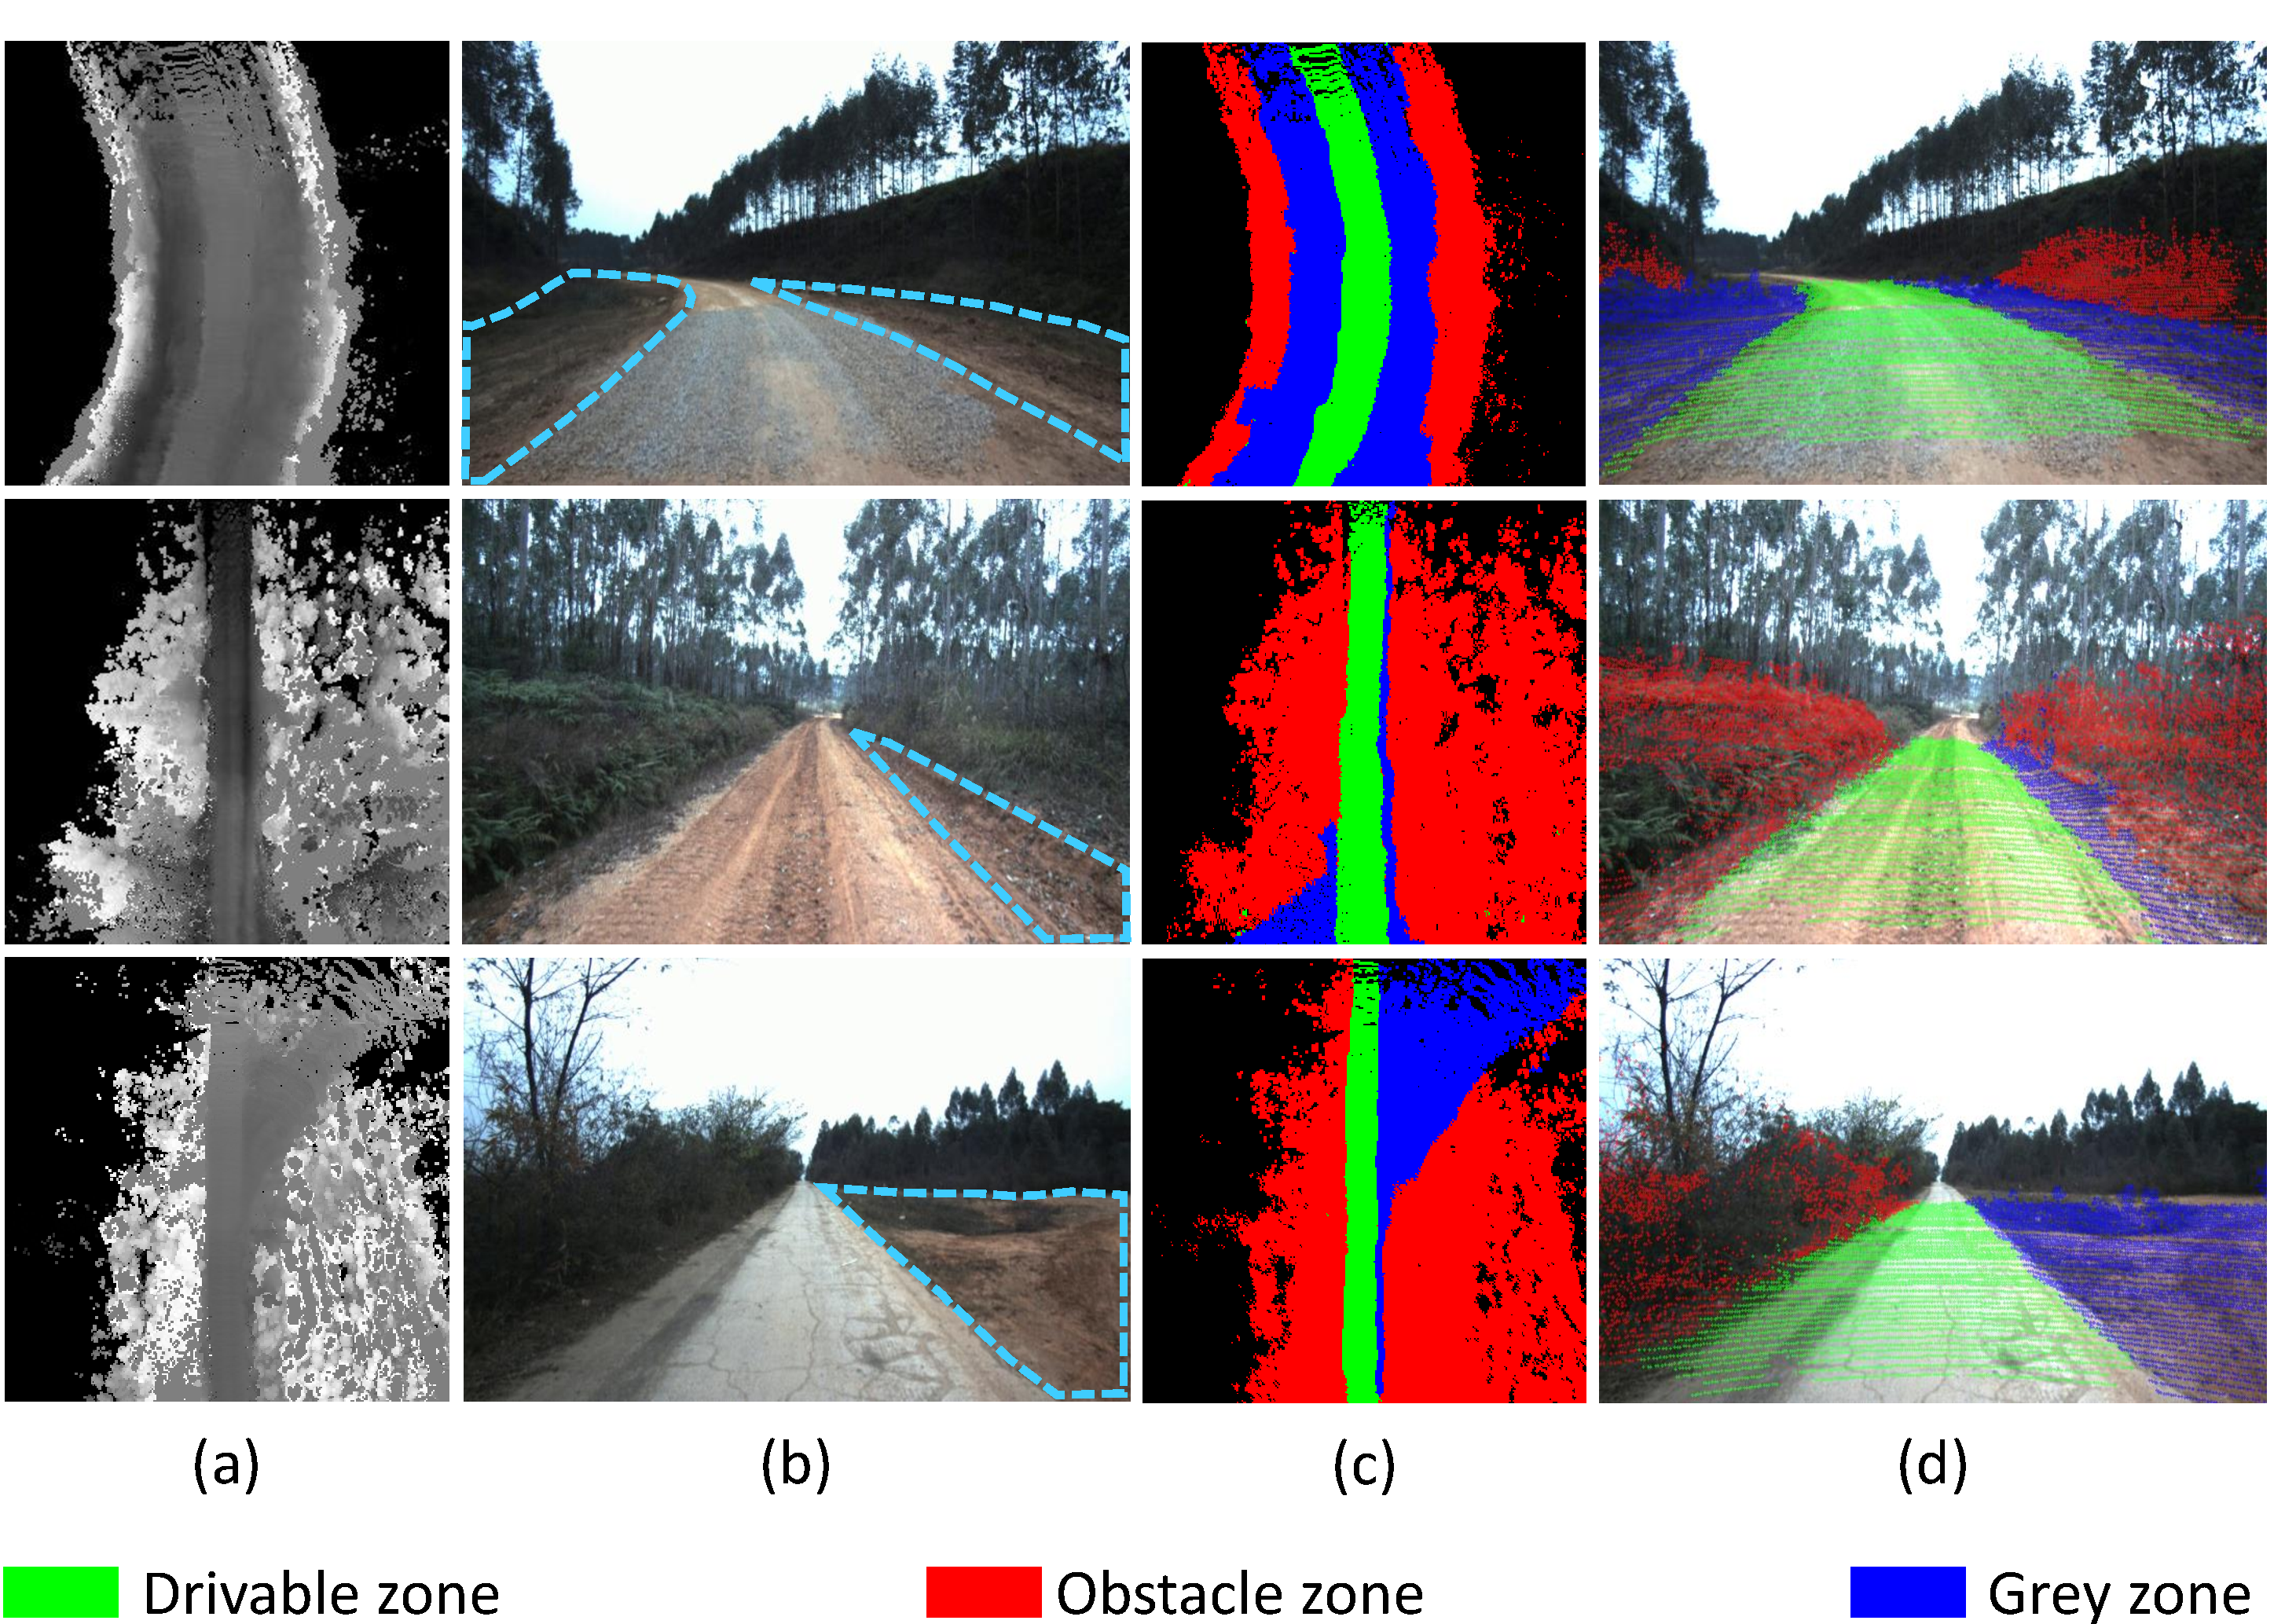
\includegraphics[scale=0.17]{offRoadExample.pdf}
	\caption{The ambiguities in off-road drivable area extraction. (a) Input LiDAR data in bird's-eye view (the ego-car is in the center of the image with upward heading). (b) Image reference of input data. (c) Human annotation. (d) Projected point clouds in camera coordinate.}
	\label{fig:example}
\end{figure}

\section{RELATED WORKS}	\label{sec:relatedworks}
Camera is one of the most important sensors in the road/drivable area extraction tasks for autonomous vehicles. Some camera-based methods depend on the assumption of global road priors such as the road boundaries\cite{Yuan2015}, % ?? ????
traffic lanes\cite{Aly2014}\cite{ZuWhanKim2008} or % ?? ???
vanish points\cite{Alvarez2014}\cite{Audibert2010}% ?? ???
. Some other researches do not rely on the these assumptions, but view the drivable area extraction as a segmentation of road and non-road regions\cite{Mei2018}\cite{Zhou2010}.% ?? ???? SVM
Despite achieving good performance, camera-based methods are easily affected by the changing of illumination. 
The LiDAR-based methods can fill up this weakness and the high precision 3D information can be conveniently used to extract the road boundaries\cite{Zhang2010}\cite{Wijesoma2004}\cite{Zhang2018} or fit the road plane\cite{Asvadi2016}\cite{Hu2014}. For the different characters of the two sensors, LiDAR-camera fusion becomes a natural solution. For example, Dahlkamp\cite{Stanford2006} identify a nearby drivable area by LiDAR and use it to train an image-based classifier for far-range drivable area detection.

The existing drivable area extraction methods are mostly designed for the urban environment, but the problem in off-road environment is quite different. One fundamental problem is the ambiguous definition of the drivable area, as shown in Figure.\ref{fig:example}. Many researches proposed similar concepts for the off-road scenes from their own perspectives, such as traversability analysis\cite{Suger2015} and drivable corridors\cite{Nefian2006}.
Despite some methods have already been implemented to the off-road environment\cite{Audibert2010}\cite{Stanford2006}\cite{Nefian2006}, they still have some limits. These methods usually focus on the mechanically drivable area but seldom distinguish whether these areas are likely to be chosen by a human driver, which makes great sense for autonomous vehicles.

Recently, many deep learning methods achieve impressive results on the related task\cite{barnes2017find}\cite{Han2018}\cite{Oliveira2016}\cite{chen2015deepdriving}\cite{Bellone2018}. Compared to the traditional methods, deep networks can learn high level semantic features from the data directly, which usually performs better than human-designed features.
However, the deep learning methods usually rely on large quantities of human-annotated data set like KITTI\cite{geiger2013vision} and Cityscapes\cite{cordts2016cityscapes}. For off-road environment, there is few widely-used data set for the drivable area extraction due to the ambiguous problem definition. 
In order to reduce the demand of human annotation, a few researches use a simulator to access endless data for training\cite{chen2015deepdriving}. And other researches focus on weakly-supervised\cite{barnes2017find} or semi-supervised methods\cite{Suger2015}, trying to utilize the auto-generated weakly labels, which can be easily accessed, as substitution.

This work focuses on the drivable area extraction in off-road environment. We propose a LiDAR-based deep learning framework specific to the ambiguities in this task. To reduce the demand of human-annotated data set, we also propose weakly-supervised and semi-supervised methods to learning features from auto-generated labels.

\section{METHODOLOGY}	\label{sec:method}

\subsection{Problem Definition}

Let's denote the origin point clouds from 3D LiDAR sensor as $PC={\{pt_i\}}_{0\le i<N}$, where $N$ is the number of points. We aggregate a few frames' point clouds to get a dense bird's-eye view height map $X=\{x_{j,k}\}_{0\le j<H,0\le k<W}$, which is used as our input data format. The input height map is in the size of $H\times W$ and each pixel $x_{j,k}$ means the physical height of pixel $(j,k)$. The car is in the center of $X$ with upward heading. The examples of input can be seen in Figure.\ref{fig:example}(a).

Different from the well-defined road borders in structured urban environment, the main peculiarity in off-road environment is the ambiguous area beside the road margin, which is called grey zone. In order to distinguish it with others, we let $Label Set=\{unknown,drivable\ zone,obstacle\ zone,grey\ zone\}$, and we use $G=\{g_{j,k}\}_{0\le j<H,0\le k<W}$ to denote human annotated ground truth, where $g_{j,k}\in LabelSet$.

The origin output of our proposed framework is a cost map $C=\{c_{j,k}\}_{0\le j<H,0\le k<W}$, where each $c_{j,k}\in [0,1]$ evaluates the traversability cost of pixel $(j,k)$. Our proposed framework learns a mapping from input $X$ to cost map $C$.

\begin{equation}
f_\theta^*:x_{j,k}\rightarrow c_{j,k} \in [0,1]
\end{equation}

For the convenience of comparison with human-annotated ground truth $G$ and other baseline methods, we use $d_\alpha$ to remap cost map $C$ to label $Y=y_{j,k}\in LabelSet$.

\begin{equation}
d_\alpha:c_{j,k}\rightarrow y_{j,k} \in LabelSet
\end{equation}

Therefore, the problem of this work can be formulated as learning a multi-class classifier $f_\theta=d_\alpha(f_\theta^*)$ that maps input $x_{j,k}$ to a label $y_{j,k}\in LabelSet$.

\subsection{Network Architecture}
Due to the ambiguity of the grey zone, we hold the view that classifying it as an independent label from the others is not reasonable enough. In some cases, the grey zone is drivable technically but not human-desired, which is very close or even overlapped with the drivable zone in feature space. In other cases, the grey zone may have higher traversability cost than common drivable zone, which is closer or even overlapped with the obstacle zone in feature space. As a result, viewing the ambiguous grey zone as an independent label in training process will cause confusion for the deep learning model, and the experimental results in Section.\ref{sec:experiment} give the evidence of this viewpoint.

\begin{figure}[b]
	\centering
	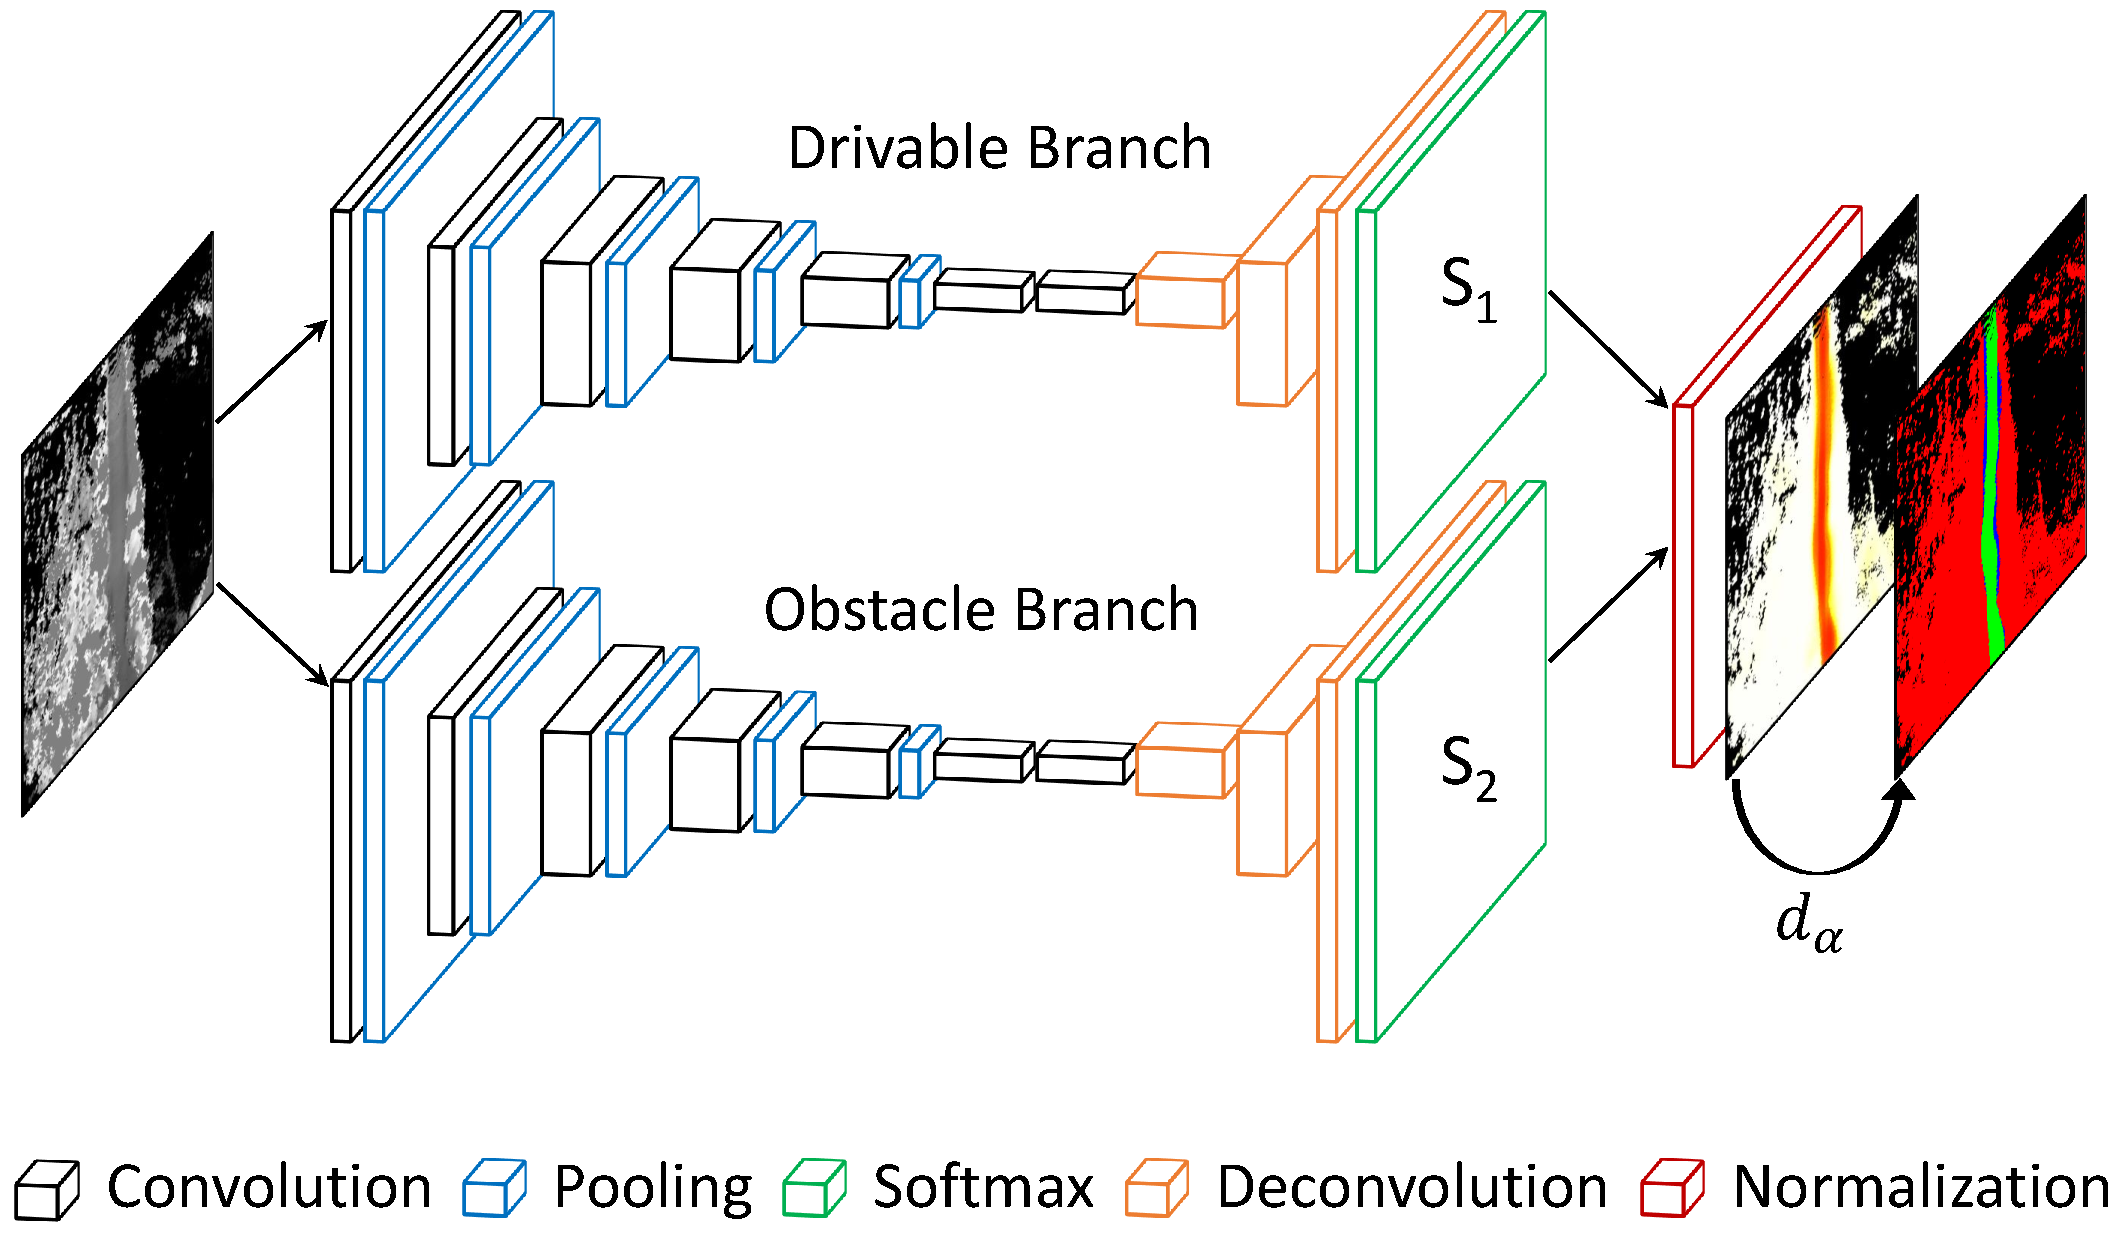
\includegraphics[scale=0.22]{network.pdf}
	\caption{The proposed network}
	\label{fig:network}
\end{figure}

\begin{figure*}[ht]
	\centering
	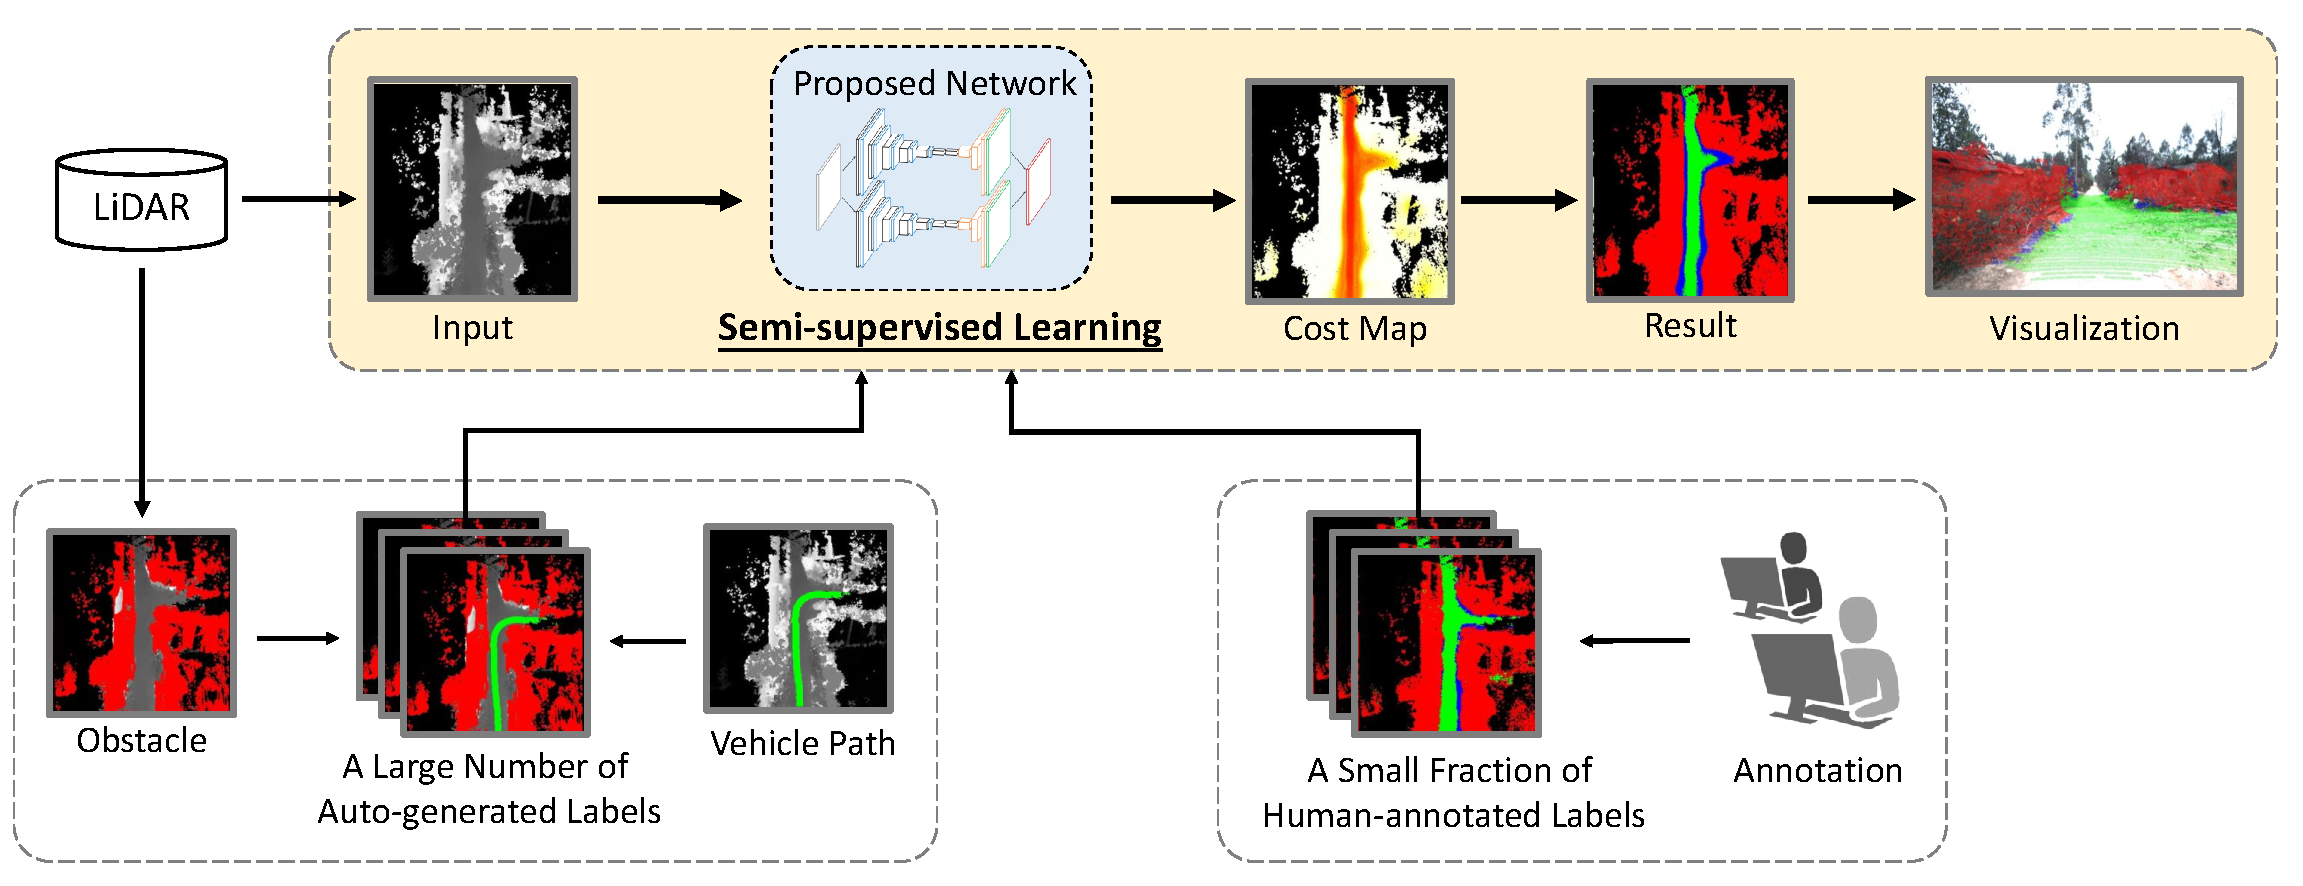
\includegraphics[scale=0.4]{framework.pdf}
	\caption{Overview of the proposed off-road drivable area extraction framework}
	\label{fig:framework}
\end{figure*}
Therefore, we can assume that the samples of grey zone are distribute between the drivable samples and the obstacle samples in feature space. The key idea of our proposed method is learning two classification surfaces in feature space and use the margin between them to split the grey zone samples. One classification surface is used to separate the drivable zone samples from others. The other one is used to separate the obstacle zone samples. We can evaluate the traversability cost of a sample by its feature distance to the two surfaces.

As shown in Figure.\ref{fig:network}, the proposed network has two branches in order to learn the two classification surfaces mentioned above. Both of them are designed according to the common VGG-based fully convolutional network. The difference is that the last layer does not output the discrete labels but the probabilistic predictions from the last softmax layer. We denote them as $S_1$ and $S_2$, which are in the range of $[0,1]$.

Each branch is trained end-to-end guided by the following cross entropy loss function:

\begin{equation}
\label{equ:loss0}
L^{br}(X;\Theta^{br})=-\sum_{i}{y_i^{br} \log{P(y_i^{br}|\Theta^{br})}}, \ br \in \{dri, obs\}
\end{equation}

where $br\in\{dri, obs\}$ is the name of network's branch. $P(y_i^{br}|\Theta^{br})$ is the probability that  pixel $i$ is predicted as label $y_i^{br}$ with the network parameters $\Theta^{br}$. We use $dri,obs$ and $gre$ to represent $drivable, obstacle$ and $grey\ zone$.

When training the network, different label $y_i^{br}$ is used in the two branches. 

\begin{equation}
y_i^{br}= 
\left\{
\begin{array}{ll}
\Psi(\vec{br}), &\quad if \ g_i = gre \\ 
\vec{g_i}, &\quad if \ g_i \in \{dri,obs \} \\
\end{array}
\right.
\end{equation}

where $\vec{br}$ is the one-hot vector of label $br\in\{dri, obs\}$. $\Psi(\vec{dri})=\vec{obs}$ and $\Psi(\vec{obs})=\vec{dri}$. For example, we replace all the pixels with ground truth $g_i=gre$ to the label $obs$ to get $y_i^{dri}$ when training the drivable branch.

We use the following regulation to calculate the traversability cost map $C$ and the discrete label:

\begin{equation}
C= 
\left\{
\begin{array}{ccc}
S_1, &\  if \ S_1>\alpha_1 \\ 
1-S_2, &\ if \ S_2>\alpha_2 \\
\frac{1-S_2}{1-S_1 + 1-S_2}, &\ otherwise
\end{array}
\right.
\end{equation}

where the pixels satisfied the first condition will be labeled as $y_{j,k}=dri$, the second is $y_{j,k}=obs$ and the last is $y_{j,k}=gre$.

\subsection{Weakly- and Semi-supervised Learning}

In order to reduce the demand of the high-cost human-annotated data, we propose a semi-supervised learning method shown in Figure.\ref{fig:framework}. For our weakly-supervised method, there will not be human-annotated labels using for training. And for our semi-supervised method, this framework can combine a large number of auto-generated labels (see Section.\ref{sec:autolabel} for more details) and only a small fraction of human-annotated labels to train the network. Except the numerous auto-generated labels, this framework is almost the same as the fully-supervised one. Our proposed network receives the LiDAR-based height maps as the inputs and outputs the traversability cost map for each pixel. For the convenience of evaluation, the cost map will be discreted to the 3-class result and combined with the image for visualization.

For human-annotated data $X_h$, we use the loss function Equation (\ref{equ:loss0}) for training. For data $X_w$ with only auto-generated weakly labels, we define the loss  $L_{semi}^{br}$ in branch $br$ as below:

\begin{equation}
\label{equ:loss1}
L^{br}_{semi}(X_w;\Theta^{br})=-\lambda \sum_{i}{\widetilde{y_i^{br}} \log{P(\widetilde{y_i^{br}}|\Theta^{br})}}
\end{equation}

where $\lambda$ is a regularization weight. $\widetilde{y_i^{br}}$ is used for weakly- and semi-supervised training, which has a similar definition as $y_i^{br}$ except for the pixels without auto-generated labels $\widetilde{g_i}$. $unk$ means the unknown zone.

\begin{table*}
	\caption{Evaluation Measures}
	\label{tab:evaluation}
	\centering
	\renewcommand{\arraystretch}{1.7}
	\begin{tabular}{cclccl}
		\hline
		\multicolumn{3}{c|}{Drivable Zone}                                                                                                    & \multicolumn{3}{c}{Obstacle Zone}                                                                                                  \\ \hline
		Definition                                            & \multicolumn{2}{c|}{Explanation}                                               & Definition                                          & \multicolumn{2}{c}{Explanation}                                               \\ \hline
		$Q_1={TP(G_{dri})}/{\Arrowvert Y_{dri} \Arrowvert}$   & \multicolumn{2}{c|}{$TP(G_{dri})=\Arrowvert G_{dri}\cap Y_{dri} \Arrowvert$}   & $Q_1={TP(G_{obs})}/{\Arrowvert Y_{obs} \Arrowvert}$ & \multicolumn{2}{c}{$TP(G_{obs})=\Arrowvert G_{obs}\cap Y_{obs} \Arrowvert$}   \\
		$Q_2={TP(G_{dri})}/{\Arrowvert G_{dri} \Arrowvert}$   & \multicolumn{2}{c|}{$TP(G_{dri})=\Arrowvert G_{dri}\cap Y_{dri} \Arrowvert$}   & $Q_2={TP(G_{obs})}/{\Arrowvert G_{obs} \Arrowvert}$ & \multicolumn{2}{c}{$TP(G_{obs})=\Arrowvert G_{obs}\cap Y_{obs} \Arrowvert$}   \\
		$Q_3={TP(VP_{dri})}/{\Arrowvert VP_{dri} \Arrowvert}$ & \multicolumn{2}{c|}{$TP(VP_{dri})=\Arrowvert VP_{dri}\cap Y_{dri} \Arrowvert$} & /                                                   & \multicolumn{2}{c}{/}                                                         \\
		$F_1={2Q_1Q_2}/{(Q_1+Q_2)}$                           & \multicolumn{2}{c|}{$F_1$ measure}                                            & $F_1={2Q_1Q_2}/{(Q_1+Q_2)}$                         & \multicolumn{2}{c}{$F_1$ measure}                                             \\ 
		\hline
	\end{tabular}
	\renewcommand{\arraystretch}{2.3}
	\begin{tabular}{llllll}
		\textbf{dri}: Drivable zone                 & \textbf{obs}: Obstacle zone              & \textbf{G}: Ground truth                            & \textbf{Y}: Prediction & \textbf{VP}: Vehicle path & $\Arrowvert \textbf{X}\Arrowvert$: Pixel number in X \\
	\end{tabular}
\end{table*}

\begin{equation}
\widetilde{y_i^{br}}= 
\left\{
\begin{array}{ll}
\Psi(\vec{br}), &\quad if \ \widetilde{g_i} = unk\ \&\ g_i \neq unk \\ 
y_i^{br}, &\quad otherwise \\
\end{array}
\right.
\end{equation}

When training the network with human-annotated labels and auto-generated labels simultaneously, combine the Equation (\ref{equ:loss0}) and Equation (\ref{equ:loss1}) together.

\begin{equation}
\label{equ:loss2}
L^{br}(X_h,X_w;\Theta^{br})=L^{br}(X_h;\Theta^{br})+L^{br}_{semi}(X_w;\Theta^{br})
\end{equation}

In each training batch, the human-annotated and auto-generated data will be randomly fed to the model, and the mean loss of them will be calculated for back propagation. If only use auto-generated label for training (weakly-supervised learning), Equation (\ref{equ:loss0}) will be the loss function.

\section{IMPLEMENTATION DETAILS} \label{sec:implementationdetails}

\subsection{Automatic Labeling}	\label{sec:autolabel}

As illustrated in Figure.\ref{fig:framework}, we make use of amounts of recorded data from the data collection car to achieve the auto-generated labels.
We follow a rules-based region grow method described in Algorithm.\ref{alg:rg} to generate the vertical obstacles from LiDAR data as the weakly obstacle zone labels. Only need to set a loose threshold for region grow, we can get a relatively strict vertical obstacle area.

Besides, we assume the vehicle path chosen by the human driver must belong to the drivable zone. So we project the data collection car's GPS trajectories with the same width as the car to the input height map, and they are labeled as the weakly drivable zone.

\begin{algorithm}	
	\caption{Region Grow}
	\label{alg:rg}
	\begin{algorithmic}[1]
		\Require Height map $X$, Height threshold $T_h$, Angle threshold $T_a$, Initial road height threshold $T_r$
		\Ensure Drivable region set $S_d$, Obstacle region set $S_o$
		\State Initialize: waiting list $Q=\emptyset,S_d=\emptyset,S_o=\emptyset$
		\State Delta height function: $\Delta H$
		\State Delta angle function: $\Delta A$
		\ForAll {$x_i$ \textbf{in} $X$}
		\If {$x_i \in [-T_r,T_r]$}
		\State $Q \gets Q \cup x_i$, $S_d \gets S_d \cup x_i$
		\EndIf
		\EndFor
		\While {$Q \neq \emptyset$}
		\ForAll {$x_j \in NeighbourSet(x_i)$}
		\If {$\Delta H(x_i,x_j) < T_h$ \textbf{and} $\Delta A(x_i,x_j) < T_a$}
		\State $Q \gets Q \cup x_j$, $S_d \gets S_d \cup x_j$
		\Else
		\State $S_o \gets S_o \cup x_j$
		\EndIf
		\EndFor
		\State $Q \gets Q-x_i$
		\EndWhile
	\end{algorithmic}
\end{algorithm}

\subsection{Training Setup}
The training process and experiments are conducted on a NVIDIA TitanX GPU. The network is trained with Adam optimizer with the learning rate 1e-4 and the batch size of 16. Data augmentation is applied mainly for image rotation, because the vehicle seldom makes a turn. In semi-supervised learning loss, the regularization weight $\lambda$ is usually less than 1, such as $0.4$. When converting the cost map into discrete labels, we set the thresholds $\alpha_1$ and $\alpha_2$ to 0.5 for an SUV. Actually, they can be changed based on the through capacity of a vehicle. 

\subsection{Evaluation Measures}	\label{sec:eval}

In order to evaluate the quantitative performance of different algorithms in the off-road environment, we design some evaluation measures in Table.\ref{tab:evaluation}. 

Due to the ambiguous definition of the grey zone, we do not evaluate the performance on the grey zone samples directly, but only the drivable zone and obstacle zone samples.

\subsubsection{Precision}
We define $Q_1$ to evaluate the precision performance. For the drivable zone, $Q_1={TP(G_{dri})}/{\Arrowvert Y_{dri} \Arrowvert}$. ${\Arrowvert Y_{dri} \Arrowvert}$ means the number of pixels predicted as the drivable zone. $Q_1$ measures the percentage of extracted drivable pixels that are actually the drivable zone in the ground truth. For the obstacle zone, $Q_1$ measures the percentage of extracted obstacle pixels that belong to the obstacle zone in human annotations.
\subsubsection{Recall}
We define $Q_2$ to evaluate the recall. For the drivable zone, $Q_2={TP(G_{dri})}/{\Arrowvert G_{dri} \Arrowvert}$, where ${\Arrowvert G_{dri} \Arrowvert}$ means the pixel number of the drivable zone in the ground truth. $Q_2$ measures the percentage of the ground truth drivable zone extracted by the proposed method. For the obstacle zone, $Q_2$ is defined in the similar fashion.
\subsubsection{Accuracy}
$Q_3$ is defined only for the drivable zone, which is in order to measure the percentage of the vehicle path extracted as the drivable zone. We believe that the vehicle paths chosen by the human driver must be the area with low traversability cost relatively. Therefore, we design $Q_3$ to encourage extracting the pixels of vehicle path as the drivable zone.
\subsubsection{$F_1$ Measure}
The last but not least, the $F_1$ measure is a widely-used indicator which considers both the precision and the recall. The $F_1$ measure is the harmonic average of the precision ($Q_1$) and recall ($Q_2$). 

In this work, there are some methods tend to extract the drivable zone with narrow-width, which is similar with a vehicle path. This will lead to a very high performance of precision ($Q_1$) but lower recall ($Q_2$). Besides, there are some other methods tend to extract wider drivable zone, which will lead to higher recall ($Q_2$) but lower precision ($Q_1$). In these cases, $F_1$ measure will be considered as the most important indicator to evaluate the methods performance.

\begin{table*}[b]
	\caption{quantitative evaluation of different methods}
	\label{tab:all_result}
	\centering
	\renewcommand{\arraystretch}{1.6}
	\begin{tabular}{c|cccc|ccc}
		\hline
		& \multicolumn{4}{c|}{Drivable zone}                                & \multicolumn{3}{c}{Obstacle zone}               \\ \cline{2-8} 
		& $Q_1$ (PRE)    & $Q_2$ (REC)    & $Q_3$ (ACC)    & $F_1$          & $Q_1$ (PRE)    & $Q_2$ (REC)    & $F_1$          \\ \hline
		3-class FCN (fully-sup.) & 74.93          & 82.99          & \textbf{98.92} & 78.75          & 94.36          & \textbf{98.44} & 96.36          \\
		Ours (fully-sup.)        & \textbf{76.01} & \textbf{86.72} & 98.09          & \textbf{81.01} & \textbf{96.20} & 96.75          & \textbf{96.47} \\ \hline
		RG-FCN (weakly-sup.)     & 59.78          & {79.15}        & 93.16          & 68.11          & 94.46          & {95.38}        & 94.92          \\
		Oxford PP (weakly-sup.)  & \textbf{97.00} & 47.38          & 83.71          & 63.66          & \textbf{98.40} & 89.84          & 93.93          \\
		Ours (weakly-sup.)       & 72.38          & 78.83          & {95.21}        & {75.47}        & {96.31}        & 94.84          & {95.57}        \\
		Ours (semi-sup.)         & {81.73}        & \textbf{81.73} & \textbf{96.24} & \textbf{81.73} & 95.60          & \textbf{97.38} & \textbf{96.49} \\ \hline
	\end{tabular}
\end{table*}

\section{EXPERIMENTAL RESULTS}	\label{sec:experiment}

\subsection{Data Set}
% ??785m  train: 1176   val:294    test:491
We build a typical off-road data set by our data collection vehicle, which is equipped by a Velodyne HDL-64 LiDAR, a front-view monocular camera and a GPS/IMU system. To get the input data $X$, We project point clouds captured by the LiDAR into birds-eye view. The position and posture information captured by the GPS/IMU system are required during the projection process. Besides, we use the GPS/IMU system to record the vehicle trajectory for the automatic labeling of vehicle path. We emphasize that the camera data are only used for visualization.

During the process of data collection, the vehicle is driven by a human driver and all kinds of data are time-synchronized. The input height map $X$ is in the size of $300\times 300$ with 0.2 meters pixel size. The height value of each pixel is linear projected to an integer in $[0,255]$.

The whole data set contains 1961 frames data. It's approximately about 785 meters driving distance. We choose 1176 frames for model training, 294 frames for validation and 491 frames for test.

\subsection{Proposed Method Results}
In order to evaluate our proposed method performance, we firstly compare it with a fully-supervised method to prove the reasonability of our model design for the grey zone. Except the specific design for off-road scene, another advantage of our model is that it's also suitable for weakly- and semi-supervised learning. So we then compare our weakly- and semi-supervised results with other baselines.

Figure.\ref{fig:cross_road} and Figure.\ref{fig:straight_road} show the qualitative test results of different methods in two typical scenes: a cross road scene and a straight road scene. It's necessary to mention that the cost maps of other baseline methods are directly remapped from their output labels, which only have 3 discrete values.

We use the evaluation measures described in Section.\ref{sec:eval} to compare the quantitative performance of different methods, which is shown in Table.\ref{tab:all_result}. 

\begin{figure*}[ht]
	\centering
	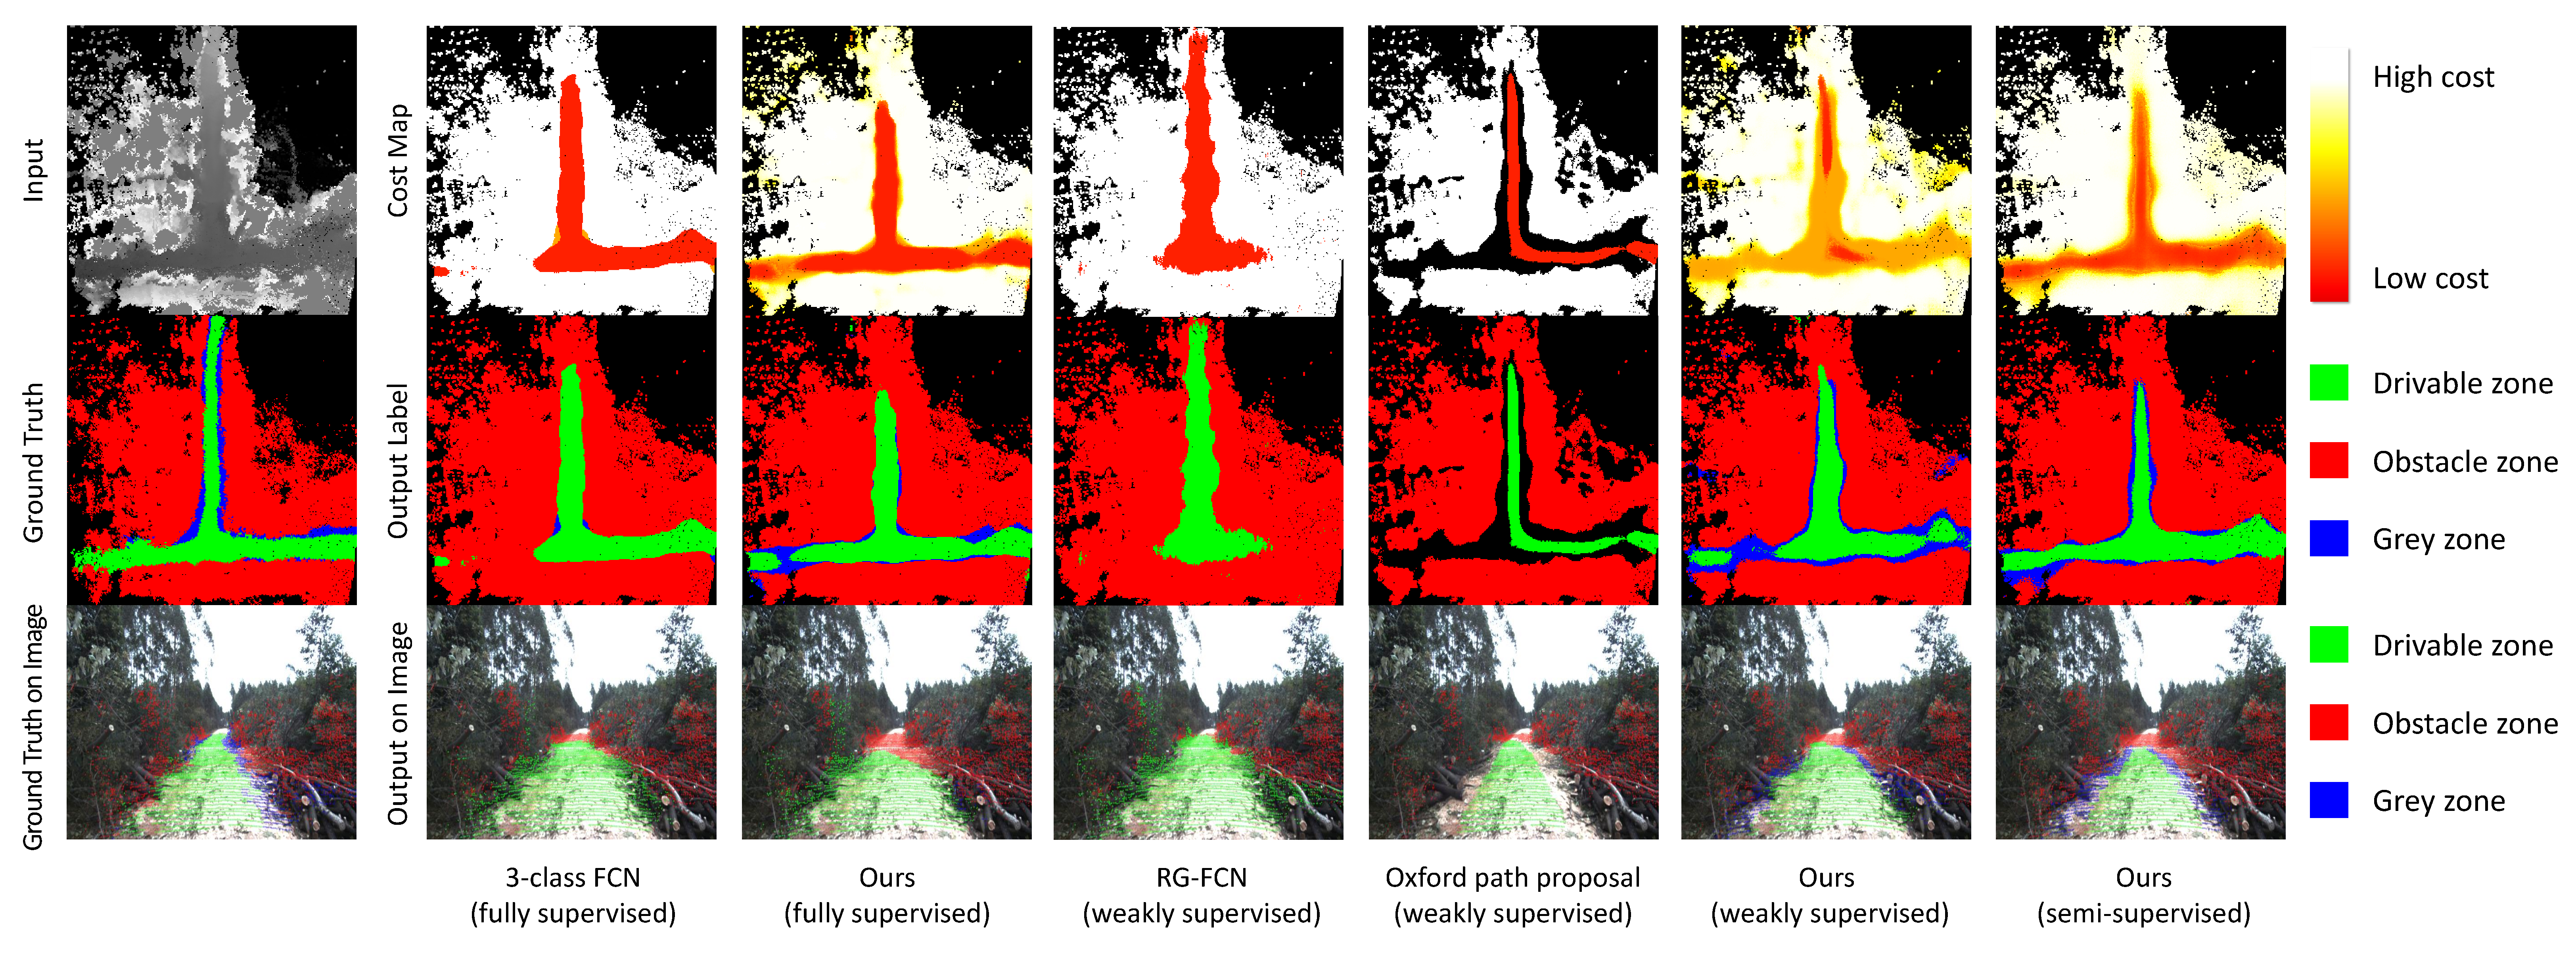
\includegraphics[scale=0.15]{crossRoad.pdf}
	\caption{Qualitative results at cross road scene.}
	\label{fig:cross_road}
\end{figure*}
\begin{figure*}[ht]
	\centering
	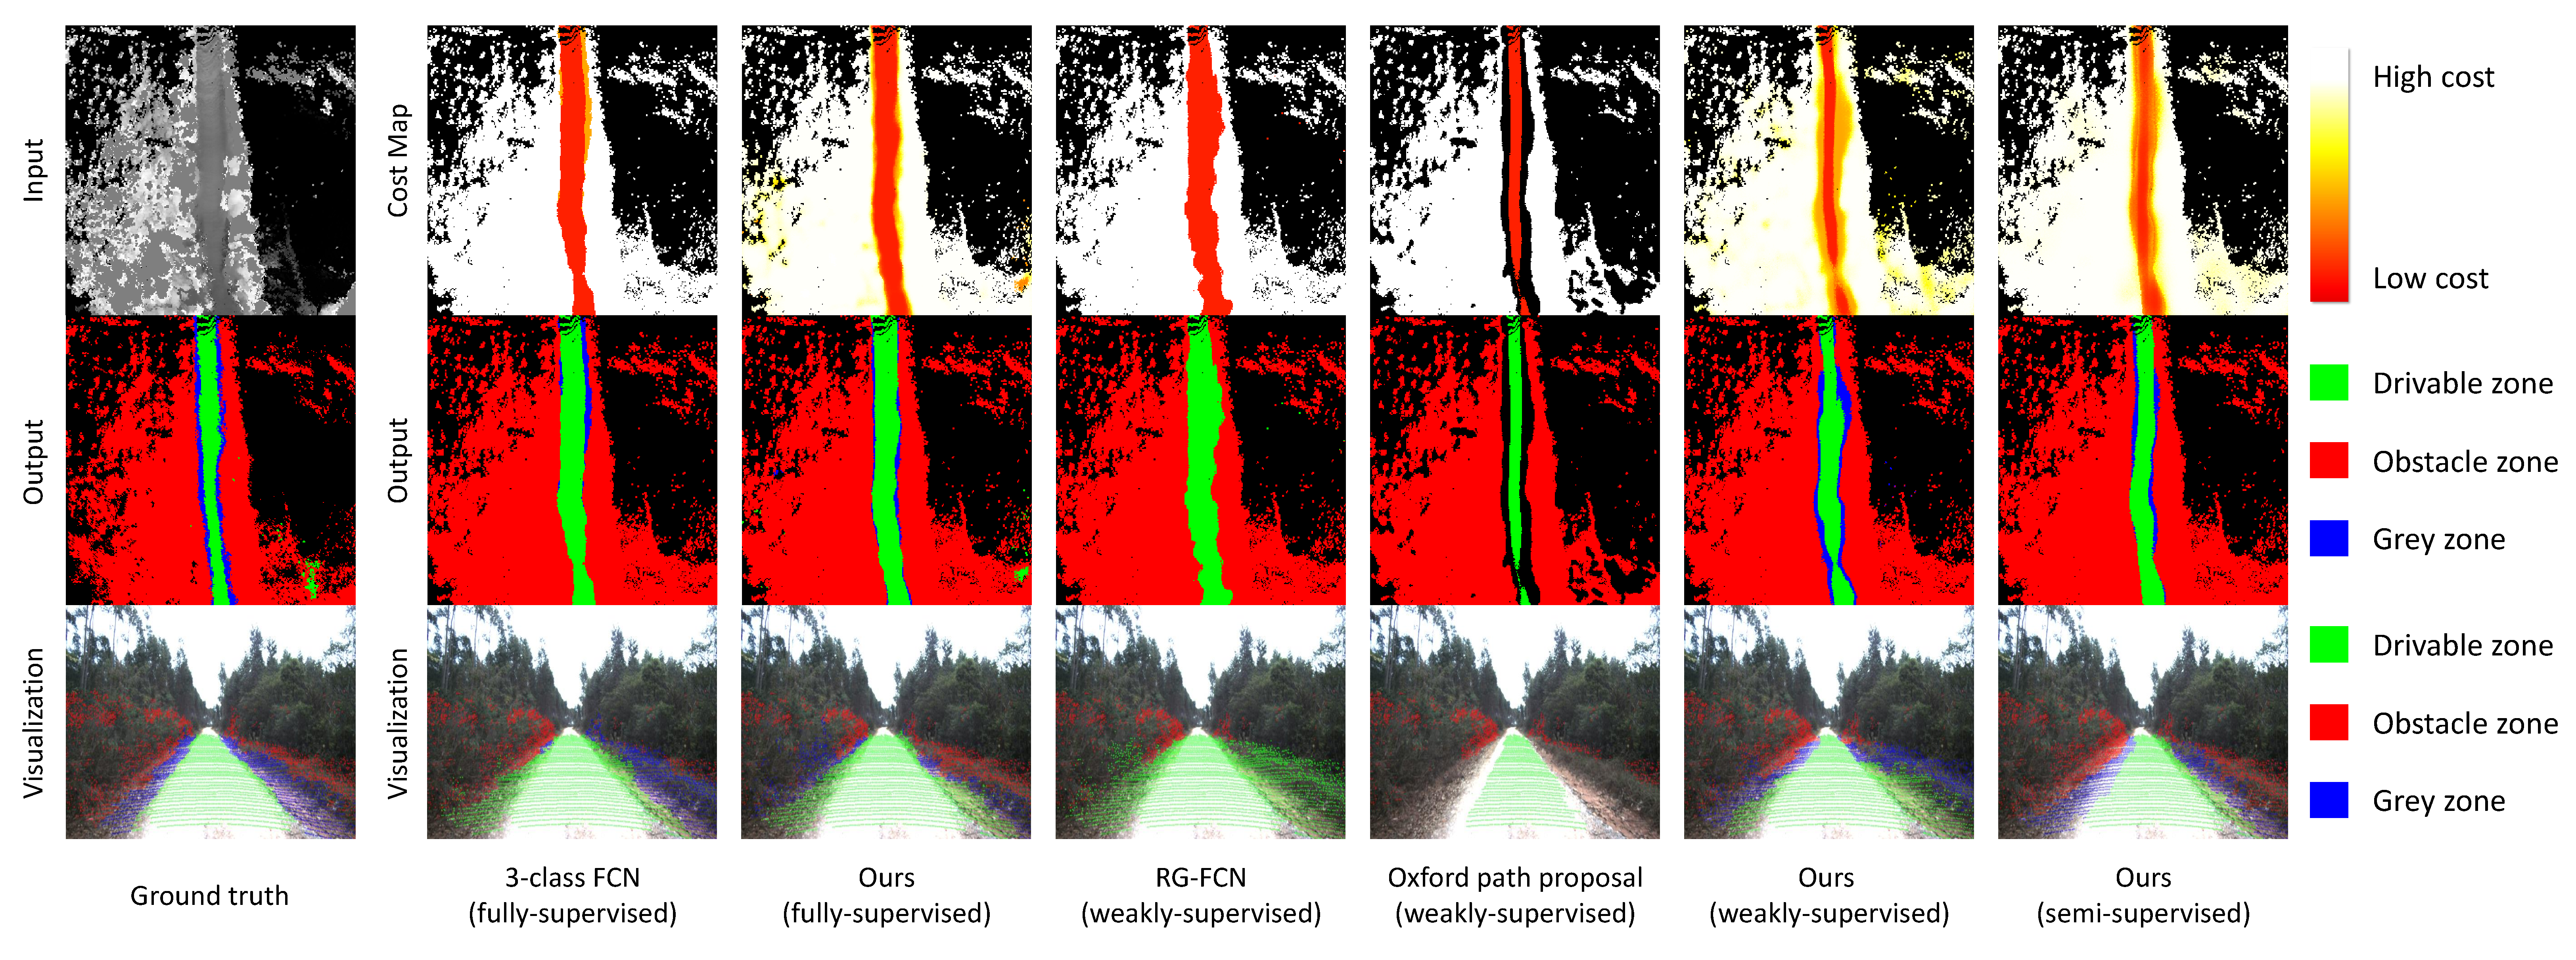
\includegraphics[scale=0.15]{straightRoad.pdf}
	\caption{Qualitative results at straight road scene.}
	\label{fig:straight_road}
\end{figure*}
\subsubsection{Fully-supervised Results}
Fully-supervised results use the human-annotated ground truth for model training. The baseline method '3-class FCN' is a fully convolutional network with the same depth as either branch in our proposed network. It treats the problem as a common 3 class classification. Our proposed fully-supervised method achieves better performance than '3-class FCN' in most evaluation measures.

We can see the first three columns in Figure.\ref{fig:cross_road} for a more concrete example. Our fully-supervised method is robuster than the common 3-class classification method in the complex cross road scene. The baseline '3-class FCN' misclassifies the left side cross road as the obstacle zone and our method successfully extract the whole structure of this cross road.


\subsubsection{Weakly-supervised Results}
The weakly-supervised method means all data for model training are auto-generated weakly labels.

%We introduce two baseline methods for comparison. The first one is denoted as 'RG-FCN', which uses a traditional rule-based region grow algorithm to generate weakly labels. These auto-generated weakly labels are used to train a FCN with a common cross-entropy loss. The second one 'Oxford path proposal' has a different way to generate the weakly labels. This method\cite{barnes2017find} is original designed for the path proposal task based on image data, which projects the vehicle path to the camera coordinate as the drivable zone and gets the obstacle zone in the images by a LiDAR scanner. This method has a great performance on the KITTI dataset\cite{geiger2013vision} and the Oxford RobotCar dataset\cite{maddern20171}. Due to the lack of other LiDAR-based weakly-supervised methods, we re-implement this method in our LiDAR-based framework as another weakly-supervised baseline.

The qualitative visualization results are shown in the last four columns of Figure.\ref{fig:cross_road} and Figure.\ref{fig:straight_road}. From the visualization results, it's easy to find that the 'RG-FCN' method tends to extract a wider drivable zone than the ground truth. The rule-based method can not distinguish the drivable zone and the grey zone with a few of thresholds, so the 'RG-FCN' tends to treat the drivable zone and the grey zone which is drivable technically as the same. The 'Oxford path proposal' results are almost to the contrary, which have very narrow drivable zone. This method can extract the drivable zone similar to the vehicle path, but the fundamental defect is too many pixels between this narrow drivable zone and the obstacle zone are labeled as unknown. A large percentage of these pixels are actually drivable and an accurate prediction of them makes a great sense for autonomous vehicles. Compared with these two baseline methods, our weakly-supervised method has obviously better performances in extraction of the drivable area. In addition, it's also as robust as the fully-supervised method in the cross road scene.

The quantitative analysis shows that our weakly-supervised method can extract the drivable area more accurately than others. Despite one baseline method has a higher precision $Q_1$ and the other one has a little higher recall $Q_2$, they both get very poor performance of the other evaluation measure. In other words, our method is the most balanced one, so we can get the $F_1$ measure that 7.4\% higher than the 'RG-FCN' and 11.8\% higher than the 'Oxford path proposal' method.

\subsubsection{Semi-supervised Results}
The semi-supervised methods means a proportion of human-annotated and auto-generated data are used for training at the same time. By the way, no matter how many human-annotated labels are contained, we will use all weakly labels for training, cause for their quite low generating cost.
We list the semi-supervised result using half human-annotated labels for training as a representative in Table.\ref{tab:all_result}. The $F_1$ measure of our semi-supervised method (81.73\%) achieves an impressive improvement compared to other baseline methods and even higher than the fully-supervised result.
It achieves better evaluations than other methods in all measures except the precision $Q_1$, the explanation of this is similar with the weakly-supervised ones. 

\begin{figure}[h]
	\centering
	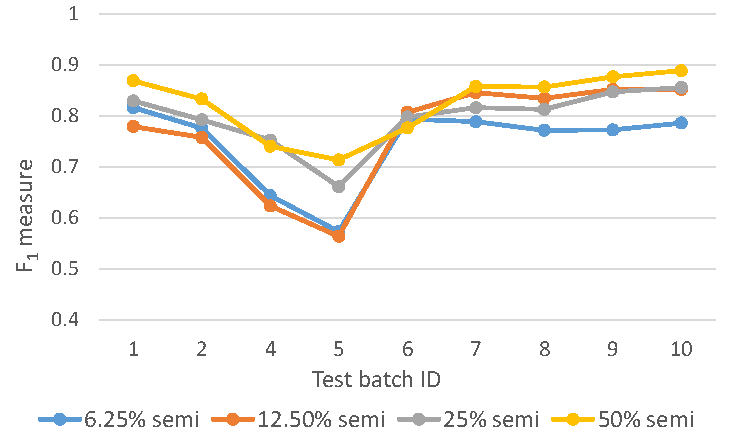
\includegraphics[scale=0.6]{semiSupvisedResult.pdf}
	\caption{Detailed comparison of semi-supervised methods on the test set.}
	\label{fig:semi_curve}
\end{figure}
\begin{table*}
	\caption{$F_1$ measure of different methods}
	\label{tab:semic}
	\centering
	\renewcommand{\arraystretch}{1.6}
	\begin{tabular}{c|ccccc}
		\hline
		- & 6.25\% semi-sup. & 12.5\% semi-sup. & 25\% semi-sup. & 50\% semi-sup. & Fully-sup.	\\
		\hline
		$F_1$ measure & 73.86 & 75.04 & 78.96 & \textbf{81.73} & 81.01 	\\
		\hline
	\end{tabular}
\end{table*}

In order to explore how the ratio of human-annotated labels influence our model performance. We compare the semi-supervised methods using different ratio's human-annotated labels, base on the key indicator $F_1$ measure. The detailed performance on the test set can be seen in Figure.\ref{fig:semi_curve}. We split the test set into 10 batches and evaluate on them respectively. The quantitative results is shown in Table.\ref{tab:semic}. The percentage in the front of 'semi-sup' means the ratio of human-annotated labels used for training. The $F_1$ measure of the 50\% semi-supervised version is higher than the fully-supervised method, and the 25\% semi-supervised version achieves higher performance than the '3-class FCN' baseline with only a quarter of human-annotated labels. It shows that our proposed semi-supervised method can significantly reduce the demand of high-cost human annotations.

\section{CONCLUSION}   \label{sec:conlusion}
In this paper, we propose a deep learning framework for off-road drivable area extraction. The proposed network structure is specifically designed for the ambiguous grey zone in the off-road environment. We also propose an automatic labeling method which generates quantities of weakly labels from the data collection vehicle's driving. It can significantly reduce the demand of human-annotated data for the weakly- and semi-supervised network training.
Crucially, it's demonstrated that the proposed semi-supervised method can achieve better performance than the fully-supervised one with even less human-annotated labels. In this work, the camera images are only used for visualization, but they actually include many useful features for the drivable area extraction, such as the colors and texture. We plan to fuse the camera information into our framework and enhance the robustness of far-field drivable area extraction in the off-road environment.

%\addtolength{\textheight}{-21cm}   % This command serves to balance the column lengths
% on the last page of the document manually. It shortens
% the textheight of the last page by a suitable amount.
% This command does not take effect until the next page
% so it should come on the page before the last. Make
% sure that you do not shorten the textheight too much.

\bibliography{refs}

\end{document}
